\section{Quantitative Violation Semantics}
The basic restriction of the forward-looking tight satisfaction semantics, as defined in the previous section, resides in its binary and prefix-closed nature.
In that framework, the monitoring process halts definitively at the first tight violation.
Despite being computationally efficient for stopping compliance systems (e.g., an access control system that is failing), this ``first-fail'' approach is insufficient for post-hoc auditing or dispute resolution.
It masks the full history of non-compliance, failing to capture cumulative violations or distinct failures by multiple agents over time, a critical requirement for comprehensive legal responsibility.
To tackle this limitation, it is necessary to transition from a boolean verdict to a \emph{quantitative semantics}, changing the emphasis from the question ``Did a violation occur?'' to ``How many violations occurred, and what was their magnitude?''


\paragraph{The Challenge of Temporal Scope.}
A prerequisite for counting violations is defining the temporal window over which the contract is evaluated.
In contrast to traditional model checking, which commonly analyzes systems that are supposed to run forever, contract monitoring operates on finite, evolving prefixes.
We identify two primary strategies for defining this scope:

\begin{enumerate}
    \item \textbf{Static Pre-computation:} One might attempt to calculate a fixed duration $T$ for a contract $C$.
    However, contracts containing unbounded repetitions ($\repit{C}$) or input-dependent regular expressions (guards/triggers) do not have a statically determinable length.
   
    \item \textbf{Dynamic On-the-Fly Detection:} The alternative is to determine the contract's status dynamically at every step.
    Here, the monitor continuously computes a \emph{residual contract}—a formula representing what remains to be fulfilled given the history of events.
   
\end{enumerate}

This work adopts the \textbf{Dynamic On-the-Fly} approach.
This requires a structural tracking mechanism, which we formalize as the \emph{Contract Progress Monitor} (CPM).
The CPM acts as a derivative function: given a contract $C$ and an incoming event, it computes the contract $C'$ that must be enforced in the next time step.
Isolating the state of the contract (via the CPM) from the evaluation of compliance (via a scoring function) enables a modular framework that can track active duties, handle contrary-to-duty (CTD) transitions, and attribute blame with precision over time. The scoring function is critical in this framework, as it provides a quantitative evaluation of compliance. This approach not only determines whether obligations have been met, but also assesses the degree of compliance or non-compliance. The interaction with the CPM measures the magnitude of violations, presenting an in-depth and nuanced view of contractual adherence that improves accountability and enforcement precision.


\subsection{Contract Progress Monitor}

The core of our measurement framework is the \emph{progression function}, $\Prog$.
The consumes the current one event  and the current \emph{state of a contract} to produce the \emph{residual contract} for the subsequent step.

\begin{definition}[Contract Progression Function]
Let $\Gamma = 2^\Sigma$ be the event alphabet.
We extend the set of contracts $\mathcal{C}$ with a distinguished symbol $\emptc$, representing a \emph{discharged contract} (one that implies no further obligations).

The progression function $\Prog: \Gamma^* \times \cDL \to \cDL \cup \{\emptc\}$ is defined recursively.
For the empty trace $\epsilon$, $\Prog(\epsilon, C) := C$.
For a single event step $\trace{A}$ with $A \in \Gamma$, the function is defined on the structure of $C$ as follows.

\paragraph{Literals (State Update).}
For any literal $\ell$ (obligation, permission, or prohibition):
\[
\Prog(\trace{A}, \ell) := \emptc
\]
\emph{Rationale:} Structurally, a literal applies to a single time step.
Once the $A$ step occurs, the literal is consumed.
Whether $A$ satisfied or violated $\ell$ is immaterial to the \emph{progression} (the duty is passed); the violation is recorded separately by the quantitative scoring function defined later.


\paragraph{Conjunction (Parallel Progress).}
\[
\Prog(\trace{A}, C_1 \wedge C_2) := \Prog(\trace{A}, C_1) \wedge \Prog(\trace{A}, C_2)
\]
We assume the symbolic identity where $\emptc$ is the neutral element for conjunction: $\emptc \wedge C' \equiv C'$.


\paragraph{Sequence (Sequential Handover).}
For a sequence $C_1 ; C_2$, progression determines if the current step concludes $C_1$:
\[
\Prog(\trace{A}, C_1 ; C_2) := 
\begin{cases}
  \Prog(\trace{A}, C_1) ; C_2 & \text{if } \Prog(\trace{A}, C_1) \neq \emptc, \\
  \Prog(\trace{A}, C_2) & \text{if } \Prog(\trace{A}, C_1) = \emptc.
\end{cases}
\]
If $C_1$ is discharged by step $A$ (i.e., its residual is $\emptc$), the monitor immediately activates the first step of the next portion $C_2$.


\paragraph{Reparation (Contrary-to-Duty Branching).}
The reparation construct is unique because its structural progression depends on the satisfaction of the primary obligation.
This is the only case where $\Prog$ relies on the tight satisfaction relation ($\satt, \violt, \presat$) to determine the path:
\[
\Prog(\trace{A}, C_1 \repair C_2) := 
\begin{cases}
  \Prog(\trace{A}, C_1) \repair C_2 & \text{if } \trace{A} \presat C_1 \text{ (Pending)}, \\
  \Prog(\trace{A}, C_2) & \text{if } \trace{A} \violt C_1 \text{ (Violation $\to$ Repair)}, \\
  \emptc & \text{if } \trace{A} \satt C_1 \text{ (Satisfaction $\to$ Discharge)}.
\end{cases}
\]
If a violation occurs ($\trace{A} \violt C_1$), the primary contract is discarded, and the secondary contract $C_2$ is activated immediately for the \emph{next} step.


\paragraph{Repetition.}
Repetition unrolls the contract one step at a time:
\[
\Prog(\trace{A}, \repit{C}) := \Prog(\trace{A}, C) ; \repit{C}
\]


\paragraph{Guarded and Triggered Contracts.}
These constructs rely on regular expression matching.
\[
\Prog(\trace{A}, \guard[re]{C}) :=
\begin{cases}
  \emptc & \text{if } \trace{A} \satt \guard[re]{C} \text{ (release)}, \\
  \guard[\Prog_{re}(\trace{A}, re)]{\Prog(\trace{A}, C)} & \text{otherwise (Guard persists)}.
\end{cases}
\]
\[
\Prog(\trace{A}, \trig[re]{C}) :=
\begin{cases}
  \emptc & \text{if } \trace{A} \violt re \text{ (Trigger failed)}, \\
  C & \text{if } \trace{A} \satt re \text{ (Trigger fires)}, \\
  \trig[\Prog_{re}(\trace{A}, re)]{C} & \text{if } \trace{A} \presat re \text{ (Trigger pending)}.
\end{cases}
\]

Where the regular progress function $\Prog_{re}: 2^\Gamma \times \cDL_{re} \to \cDL_{re} $ is defined only when $\trace{A} \presat \re$ (where $\trace{A}$ is the trace consisting of the single event $A$).
 We do not need to use $\epsilon_{re}$ as we did for the contract as $\epsilon$ is already defined in the syntax of regular expression, with $\Prog_{re}(\trace{A},\epsilon):= \epsilon$ 
 \paragraph{Atomic regular expressions}
 For a set of actions $A \in \Gamma$ we have:
$Prog_{re}(\trace{A}, A') := \epsilon.$ 
  
 \paragraph{Concatenation}
For $\re \cdot \re'$, the progression is defined as:
\[
\Prog_{re}(\trace{A}, \re \cdot \re') := 
    \Prog_{re}(\trace{A}, re) \cdot re'.
\]

\paragraph{Union}
For $re \mid re'$, the progression is defined by distinguishing cases based on violation:
\[
\Prog_{re}(\trace{A}, re \mid re') := \begin{cases} 
\Prog_{re}(\trace{A}, re') & \text{if } \trace{A} \violt re ,\\
\Prog_{re}(\trace{A}, re) & \text{if } \trace{A} \violt re' ,\\
\Prog_{re}(\trace{A}, re) \mid \Prog_{re}(A, re') & \text{otherwise}.
\end{cases}
\]

\paragraph{n-repition}
For $\re^n$, with $n \in \mathbb{N}^*$ the progression is defined as:
\[
\Prog_{re}(\trace{A}, re^n) := \Prog_{re}(\trace{A},re)\cdot re^{n-1}.
\]


\paragraph{Operator $+$}
For $\re^+$, the progression is defined as:
\[
\Prog_{re}(\trace{A}, re^+) := \Prog_{re}(\trace{A}, re) \mid \Prog_{re}(\trace{A},re)\cdot re^+.
\]

Moving up for the special case of single event traces, for $\pi = \trace{A} \circ \pi'$ with
$A \in \Gamma$ the first event and $\pi' \in \Gamma^*$ the remaining suffix. Then:
\[
  \Prog(\trace{A} \circ \pi', C) :=
  \begin{cases}
    \emptc & \text{if } \Prog(\trace{A}, C) = \emptc, \\[4pt]
    \Prog\bigl(\pi',\,\Prog(\trace{A}, C)\bigr) & \text{otherwise}.
  \end{cases}
\]


\end{definition}
The helper function $\Prog_{re}$ computes the residual regular expression following an idea from Brzozowski's derivative~\cite{brzozowski1964derivatives} of the regular expression. In our case, it is tuned for the tight semantics.

\begin{lemma}[Termination]
For each finite prefix $\pi$, $\Prog(\pi, C)$ terminates in at most $ min|\pi|$ recursive steps and the worst case is considering the worst regular expression such as the guard of the use case.

\end{lemma}
To illustrate the CPM, the evolution of the residual contract under different traces is examined. The evaluation initiates with the fundamental building block of normative enforcement: the reparation.

\begin{example}[Progression of Reparation]
\label{ex:prog-repit}
Consider the basic rental reparation clause:
\[ C_3 := \obl[1]{\PAY}\ \repair\ \obl[1]{\PAYF}. \]

\noindent\textbf{Scenario 1: Compliance.}
In the first trace $\pi$, the tenant pays rent in Month 1 ($\PAY \in A_1$). Since $\trace{A_1} \satt \obl[1]{\PAY}$, the condition for discharge is met. The reparation structure collapses to $\emptc$, meaning no further obligations exist for Month 2.

    \boxalignfigure{\resizebox{0.7\textwidth}{!}{%
 
    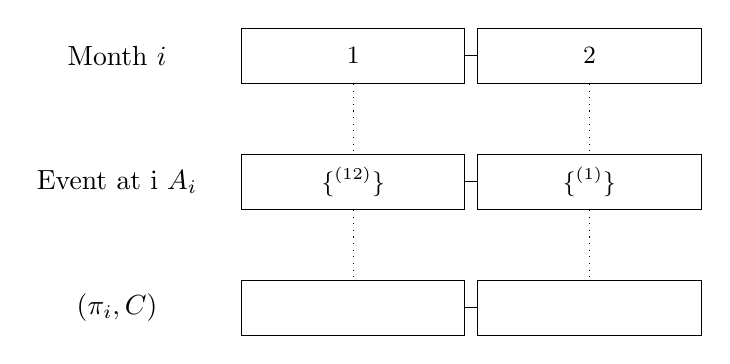
\begin{tikzpicture}[y=1.6cm,x=3.0cm]
      \tikzset{
        cell/.style={
          draw, rectangle, text width=26mm,
          minimum height=7mm, align=center, font=\small
        }
      }
    
      % Labels
      \node at (0,0)   {Month $i$};
      \node at (0,-1)  {Event at i $A_i$};
      \node at (0,-2)  {$\Prog(\pi_{i},C)$};
      % Row 1: time
      \node[cell] at (1,0) (t1) {$1$};
      \node[cell] at (2,0) (t2) {$2$};
      % Row 2: events
      \node[cell] at (1,-1) (e1) {$\{\PAY^{(12)}\}$};
      \node[cell] at (2,-1) (e2) {$\{\OCC^{(1)}\}$};
      % Row 3: residuals
      \node[cell] at (1,-2) (r1) {\emptc};
      \node[cell] at (2,-2) (r2) {\emptc};
      % Arrows
      \draw (t1)--(t2);
      \draw (e1)--(e2);
      \draw (r1)--(r2);
      % Vertical alignment
      \draw[dotted](t1.south)--(e1.north);
      \draw[dotted](e1.south)--(r1.north);
    
      \draw[dotted](t2.south)--(e2.north);
      \draw[dotted](e2.south)--(r2.north);
    \end{tikzpicture}
    }}
    {Progression on $ \obl[1]{\PAY}\ \repair\ \obl[1]{\PAYF}$ with a trace for which no reparation is  required}
    {example:prog-repair1}
    {\vspace{8pt}}{\vspace{-12pt}}

\medskip
\noindent\textbf{Scenario 2: Violation and Repair.}
In trace $\pi'$, the tenant fails to pay in Month 1 ($\PAY \notin A'_1$). Here, $\trace{A'_1} \violt \obl[1]{\PAY}$. Consequently, the CPM activates the repair branch. The residual for Month 2 becomes $\obl[1]{\PAYF}$, obliging the tenant to pay the fine.

  \boxalignfigure{\resizebox{0.7\textwidth}{!}{%
  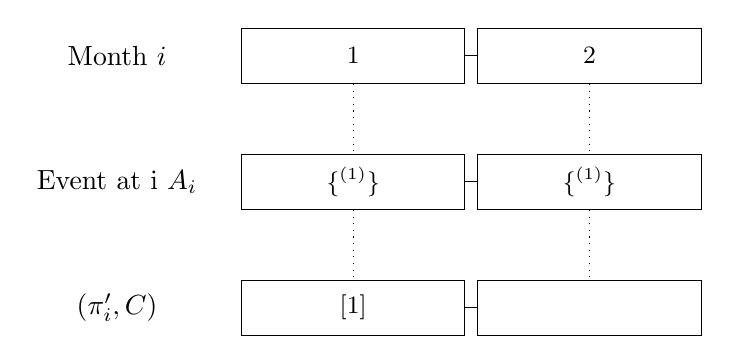
\begin{tikzpicture}[y=1.6cm,x=3.0cm]
  
    \tikzset{
      cell/.style={
        draw, rectangle, text width=26mm,
        minimum height=7mm, align=center, font=\small
      }
    }
  
    % Labels
    \node at (0,0)   {Month $i$};
    \node at (0,-1)  {Event at i $A_i$};
    \node at (0,-2)  {$\Prog(\pi'_{i},C)$};
    % Row 1: time
    \node[cell] at (1,0) (t1) {$1$};
    \node[cell] at (2,0) (t2) {$2$};
    % Row 2: events
    \node[cell] at (1,-1) (e1) {$\{\OCC^{(1)}\}$};
    \node[cell] at (2,-1) (e2) {$\{\OCC^{(1)}\}$};
    % Row 3: residuals
    \node[cell] at (1,-2) (r1) {$\obl[1]{\PAYF}$};
    \node[cell] at (2,-2) (r2) {\emptc};
    % Arrows
    \draw (t1)--(t2);
    \draw (e1)--(e2);
    \draw (r1)--(r2);
  
    % Vertical alignment
    \draw[dotted](t1.south)--(e1.north);
    \draw[dotted](e1.south)--(r1.north);
  
    \draw[dotted](t2.south)--(e2.north);
    \draw[dotted](e2.south)--(r2.north);
  
  \end{tikzpicture}
  }}
  {Progression on $ \obl[1]{\PAY}\ \repair\ \obl[1]{\PAYF}$ with a trace for which required a reparation}
  {example:prog-repair2}
  {\vspace{8pt}}{\vspace{-12pt}}
\end{example}

After establishing the evolution of single-step reparations, the analysis is extended to ongoing contracts. The following example demonstrates how the CPM handles infinite streams with recurring duties, showing how violations in one period persist into subsequent periods.

\begin{example}[Progression of Infinite Repetition]
Consider the recurring contract $\repit{C_3}$, where the tenant must pay rent (or a fine) every month.
\[ \repit{C_3} = \repit{ \obl[1]{\PAY}\ \repair\ \obl[1]{\PAYF}}. \]

\noindent\textbf{Trace Analysis.}
Consider a trace in which the tenant pays in Month 1 but fails to pay in Month 2, instead occupying the property.
\begin{itemize}
    \item \textbf{Step 1 ($A_1$):} The tenant pays. The instance of $C_3$ for Month 1 is discharged. Due to the repetition operator, the residual is $\emptc; \repit{C_3} \equiv \repit{C_3}$. The contract effectively ``resets'' for the next month.
    \item \textbf{Step 2 ($A_2$):} The tenant occupies but does not pay. The instance of $C_3$ for Month 2 violates the condition. Unlike Step 1, the residual does not reset cleanly. Instead, the violated obligation transforms into its reparation $\obl[1]{\PAYF}$, which must be fulfilled in the \emph{next} step (Month 3), alongside the continuing repetition $\repit{C_3}$.
\end{itemize}
This results in an accumulation of duties: the fine from Month 2 and the new rent for Month 3.

  \boxalignfigure{\resizebox{0.7\textwidth}{!}{%
  \begin{tikzpicture}[y=1.6cm,x=3.0cm]
  
    \tikzset{
      cell/.style={
        draw, rectangle, text width=26mm,
        minimum height=7mm, align=center, font=\small
      }
    }
  
    % Labels
    \node at (0,0)   {Month $i$};
    \node at (0,-1)  {Event at i $A_i$};
    \node at (0,-2)  {$\Prog(\pi_{i},C)$};
    % Row 1: time
    \node[cell] at (1,0) (t1) {$1$};
    \node[cell] at (2.5,0) (t2) {$2$};
    % Row 2: events
    \node[cell] at (1,-1) (e1) {$\{\PAY^{(12)}\}$};
    \node[cell] at (2.5,-1) (e2) {$\{\OCC^{(1)}\}$};
    % Row 3: residuals
    \node[cell] at (1,-2) (r1) {$\repit{C_3}$};
    \node[cell] at (2.5,-2) (r2) {$\obl[1]{\PAYF} ;$\\$ \repit{C_3}$};
    % Arrows
    \draw (t1)--(t2);
    \draw (e1)--(e2);
    \draw (r1)--(r2);
  
    % Vertical alignment
    \draw[dotted](t1.south)--(e1.north);
    \draw[dotted](e1.south)--(r1.north);
  
    \draw[dotted](t2.south)--(e2.north);
    \draw[dotted](e2.south)--(r2.north);
  
  \end{tikzpicture}
  }}
  {Progression on $\repit{C_3}$ where the obligation is met in the first month but violated in the second.}
  {example:prog-repitc1}
  {\vspace{8pt}}{\vspace{-12pt}}
\end{example}

While repetitions capture simple recurring duties, more complex contracts are often bound by conditions. The following analysis studies how the CPM handles \emph{guarded contracts}, in which the outer structure (the guard) and the inner structure (the obligations) evolve independently until a termination event occurs.

\begin{example}[Progression of Guarded Contracts] 
A guarded contract that persists until a termination notice ($\notifterm$) is issued is examined.
\[ \guard[\Gamma^+ \cdot \notifterm^{(1)}]{\repit{C_3}} \]

\noindent\textbf{Trace 1: Successful Termination.}
The tenant pays in Month 1 ($A_1$) and issues a termination notice in Month 2 ($A_2$).
\begin{itemize}
    \item At $i=1$, the event $A_1$ satisfies the inner contract $C_3$ (rent paid), but does not satisfy the guard (no notice). The residual is the guarded repetition.
    \item At $i=2$, the event $A_2$ contains $\notifterm$. This satisfies the guard expression. The CPM immediately reduces the entire contract to $\emptc$, signifying the contract has ended.
\end{itemize}

  \boxalignfigure{\resizebox{0.85\textwidth}{!}{%
  \begin{tikzpicture}[y=1.8cm,x=3.8cm]
  
    \tikzset{
      cell/.style={
        draw, rectangle, text width=34mm,
        minimum height=8mm, align=center, font=\small
      }
    }
    % Local definition for the residual regex to fit in the box
    \def\resid{\notifterm \mid \Gamma^+ \cdot \notifterm}
  
    % Labels
    \node at (0,0)   {Month $i$};
    \node at (0,-1)  {Event at i $A_i$};
    \node at (0,-2)  {$\Prog(\pi_{i},C)$};
    % Row 1: time
    \node[cell] at (1,0) (t1) {$1$};
    \node[cell] at (2.4,0) (t2) {$2$};
    % Row 2: events
    \node[cell] at (1,-1) (e1) {$\{\PAY^{(1)}, \PAY^{(2)}\}$};
    \node[cell] at (2.4,-1) (e2) {$\{\OCC^{(1)}, \notifterm^{(1)}\}$};
    % Row 3: residuals
    % Step 1: Contract satisfied (payment made), Guard not satisfied yet (needs >0 length or specific event).
    % Residual guard becomes (Notif | Gamma+ . Notif)
    \node[cell] at (1,-2) (r1) {$\guard[\resid]{\repit{C_3}}$};
    % Step 2: Guard satisfied by NotifTerm in A2. Contract discharges to epsilon.
    \node[cell] at (2.4,-2) (r2) {\emptc};
    % Arrows
    \draw (t1)--(t2);
    \draw (e1)--(e2);
    \draw (r1)--(r2);
  
    % Vertical alignment
    \draw[dotted](t1.south)--(e1.north);
    \draw[dotted](e1.south)--(r1.north);
  
    \draw[dotted](t2.south)--(e2.north);
    \draw[dotted](e2.south)--(r2.north);
  
  \end{tikzpicture}
  }}
  {Progression on guarded contract where the termination notice at step 2 discharges the contract.}
  {example:prog-guard1}
  {\vspace{8pt}}{\vspace{-12pt}}

\medskip
\noindent\textbf{Trace 2: Pending Guard with Internal Violation.}
In this scenario, the tenant pays in Month 1 but fails to pay in Month 2 (and gives no notice).
\begin{itemize}
    \item At $i=2$, the guard is \emph{not} satisfied.
    \item Simultaneously, the inner contract $\repit{C_3}$ processes the event. Since rent was not paid, the inner contract evolves into a reparation state ($\obl[1]{\PAYF}$).
    \item The resulting residual is a guarded reparation: $\guard[\dots]{(\obl[1]{\PAYF} ; \repit{C_3})}$.
\end{itemize}
This illustrates how the CPM maintains the ``wrapper'' (the guard) while the content inside (the obligations) evolves and accumulates violations independently.

  \boxalignfigure{\resizebox{0.95\textwidth}{!}{%
  \begin{tikzpicture}[y=1.8cm,x=4.4cm]
  
    \tikzset{
      cell/.style={
        draw, rectangle, text width=40mm,
        minimum height=8mm, align=center, font=\small
      }
    }
    \def\resid{\notifterm \mid \Gamma^+ \cdot \notifterm}
  
    % Labels
    \node at (0,0)   {Month $i$};
    \node at (0,-1)  {Event at i $A_i$};
    \node at (0,-2)  {$\Prog(\pi'_{i},C)$};
    
    % Row 1: time
    \node[cell] at (1,0) (t1) {$1$};
    \node[cell] at (2,0) (t2) {$2$};
    
    % Row 2: events
    \node[cell] at (1,-1) (e1) {$\{\PAY^{(1)}, \PAY^{(2)}\}$};
    \node[cell] at (2,-1) (e2) {$\{\OCC^{(1)}\}$};
    
    % Row 3: residuals
    % Step 1: Manual line break using \\
    \node[cell] at (1,-2) (r1) {$\lceil \resid \rceil$ \\ $\repit{C_3}$};
    % Step 2: Manual line break using \\
    \node[cell] at (2,-2) (r2) {$\lceil \resid \rceil$ \\ $(\obl[1]{\PAYF} ; \repit{C_3})$};
    % Arrows
    \draw (t1)--(t2);
    \draw (e1)--(e2);
    \draw (r1)--(r2);
  
    % Vertical alignment
    \draw[dotted](t1.south)--(e1.north);
    \draw[dotted](e1.south)--(r1.north);
  
    \draw[dotted](t2.south)--(e2.north);
    \draw[dotted](e2.south)--(r2.north);
  
  \end{tikzpicture}
  }}
  {Progression on a guarded contract where the guard is not satisfied, and the inner contract triggers a reparation.}
  {example:prog-guard2}
  {\vspace{8pt}}{\vspace{-12pt}}
  
\end{example}


\section{Quantitative violation semantics}
To define the quantitative violation semantics to not stop at the first violation prefix, we reuse  \emph{Contract Progress function} as the underlying state-transition mechanism.
 The progression function $\Prog$ is utilized to dynamically evolve the contract after every observation, producing a sequence of \emph{residual contracts} that represent the exact normative state at each point in time.
  By updating the contract state step-by-step, we ensure that the violation score for any given event is calculated strictly against the specific literals in force at that moment, accounting for all prior satisfactions, discharges, or triggered reparations. Then propagating the updated residual to the subsequent evaluation step.
  For each event on a trace, we define a way to evaluate only the enforced literal instead of the whole contract as an optimization step. To do so we define the function literal head.
  \begin{definition}[Literal Head]
    Let $\epsilon_\ell$ be a distinguished symbol denoting the absence of an immediately available literal.
    The \emph{literal head} function
    \[
      \LH : \cDL \to (\ell \cup \{\epsilon_\ell\})
    \]
    is defined inductively on the structure of contracts as follows:
    \[
    \begin{aligned}
    \LH(\ell) &:= \ell \\[2pt]
    \LH(C ; C') &:= \LH(C) \\[2pt]
    \LH(C \repair C') &:= \LH(C) \\[2pt]
    \LH(\trig[re]{C}) &:= 
    \begin{cases}
    \epsilon_\ell, & \text{if } re \neq \epsilon,\\
    \LH(C), & \text{if } re = \epsilon.
    \end{cases} \\[6pt]
    \LH(\guard[re]{C}) &:= 
    \begin{cases}
    \LH(C), & \text{if } re \neq \epsilon,\\
    \epsilon_\ell, & \text{if } re = \epsilon.
    \end{cases} \\[6pt]
    \LH(C^n) &:= \LH(C) \\[2pt]
    \LH(\repit{C}) &:= \LH(C).
    \end{aligned}
    \]
    \end{definition}

    We move now to define the quantitative violation semantics based on: \begin{inparaenum} \item the progress monitor returning which are the remaining parts of a contract that are still to be evaluated, \item  Scoring each event against the head literal of the residual contract returned by the $\Prog$ function. The final score of a function is thus the sum of violation for each event. \end{inparaenum}

  \begin{definition}[Quantitative Violation Semantics]
    Let $\trace{A}$ be a single event trace over $\Gamma$,  $\pi$ be a (possibly empty) finite trace $\Gamma^*$, and $C$ be a contract from $\cDL$.
    We define the \emph{quantitative violation semantics}, denoted by $\qsem{}: \Gamma^*, \cDL \to \mathbb{N} $, which maps a trace and a contract to a  natural number representing the violation score of trace on the contract. 
    The function is defined recursively by evaluating the head of the trace ($\trace{A}$) and propagating the residual contract to the tail ($\pi$):
    \[
    \qsem{\trace{A}\concat \pi, C} :=
    \begin{cases} 
      \qsem{\trace{A}, C } & \text{if } \pi = \epsilon \lor \Prog(\trace{A},C)= \emptc,\\
      \qsem{\trace{A}, C } + \qsem{\pi, \Prog(\trace{A},C)} & \text{otherwise}.
    \end{cases}
    \]
    where the \emph{instantaneous violation score} for a single event $\trace{A}$ against a contract $C$ is defined inductively on the structure of the contract:
    \[
    \qsem{\trace{A}, C} :=
    \begin{cases} 
      \qsem{\trace{A},C_1} + \qsem{\trace{A}, C_2} & \text{if } C = C_1 \wedge C_2, \\
      0 &\text{if } \lnot(\trace{A} \violt \LH(C)) \sor \LH(C)= \epsilon_{\ell}\\
      1 & \text{if } \trace{A} \violt \LH(C), \\
    \end{cases}
    \]
    \end{definition}
Intuitively, the formula $\qsem{\trace{A}\concat \pi, C}$ treats the contract execution as a path-accumulation problem. At every time step, the function:
\begin{enumerate}
    \item \textbf{Snapshots the penalty:} It calculates $\qsem{\trace{A}, C}$, which asks ``Given the current literals from$C$, does the current event $A$ violate any of them?'' This is a stateless check based purely on the structure of $C$ at that instant.
    \item \textbf{Updates the state:} It computes $\Prog(\trace{A}, C)$, effectively moving the contract pointer forward (e.g., from a paid obligation to the next month's rent, or from a violated duty to a reparation).
    \item \textbf{Accumulates:} It adds the snapshot penalty to the result of the recursive call on the remaining trace using the \emph{new} state.
\end{enumerate}

Intuitively, the formula $\qsem{\trace{A}\concat \pi, C}$ treats the contract execution as a path-accumulation problem. At every time step, the function:
\begin{enumerate}
    \item \textbf{Snapshots the penalty:} It calculates $\qsem{\trace{A}, C}$, which asks ``Given the current literals from $C$, does the current event $A$ violate any of them?'' This is a stateless check based purely on the structure of $C$ at that instant.
    \item \textbf{Updates the state:} It computes $\Prog(\trace{A}, C)$, effectively moving the contract pointer forward (e.g., from a paid obligation to the next month's rent, or from a violated duty to a reparation).
    \item \textbf{Accumulates:} It adds the snapshot penalty to the result of the recursive call on the remaining trace using the \emph{new} state.
\end{enumerate}

The explicit handling of Sequence and Reparation is done in the contract progress function, which ensures that ``zero-delay'' transitions are penalized correctly. For instance, if a contract requires $C_1$ then $C_2$, and an event discharges $C_1$ but violates $C_2$ in the same step, the summation logic ($\qsem{\trace{A}, C_1} + \qsem{\trace{A}, C_2}$) ensures the violation of $C_2$ is not ignored simply because it appeared in a continuation.


The definition of the instantaneous score $\qsem{\trace{A}, C}$ rests on distinguishing between \textbf{concurrent} (parallel) obligations and \textbf{structural} (atomic) constraints. It decouples the measurement of the ``volume'' of non-compliance from the binary verification of specific rules.

\paragraph{Additivity of Concurrency.}
The case $\qsem{\trace{A}, C_1 \wedge C_2} := \qsem{\trace{A}, C_1 } + \qsem{\trace{A}, C_2}$ captures the ``width'' of the violation as show in Example.\ref{fig:joint-blame}. In normative systems, a conjunction represents distinct, independent obligations active simultaneously. By summing the scores, the function ensures that the penalty is proportional to the number of distinct parallel duties neglected in a single instant, preventing ``violation masking'' where a single boolean verdict would hide multiple breaches.

\paragraph{Binary Structural Verdict.}
For constructs that are not distinct parallel duties (such as literals, sequences, or reparations), the definition relies on the binary tight violation relation ($\violt$). This captures the ``existence'' of a fault in a non-decomposable structure. For example, a single atomic duty ($\obl{a}$) can only be violated once per step.

\paragraph{Separation of State and Score.}
This approach assumes that the complexity of temporal evolution is handled by $\Prog$, while $\qsem{}$ handles the instantaneous cost. By reducing non-conjunction cases to a simple check ($\trace{A} \violt C$), the definition asserts that scoring is local (checking if the current active node is broken), while progression is temporal (handling the flow from one obligation to the next).


We summarize these properties in the following theorem, which establishes that the quantitative score is a monotonically increasing function that acts as a "super-set" of the binary violation semantics.
While a binary trace might be "Satisfied" (via reparation), the quantitative score reveals the cost of that path.


\begin{theorem}[Consistency of Quantitative and Tight Semantics]
  \label{thm:quant-consistency}
  For any contract $C$ and finite trace $\pi$:
  \begin{enumerate}
      \item \textbf{Zero Score Implications:}
      If $\qsem{\pi, C} = 0$, then exactly one of the following three disjoint cases holds:
      \begin{enumerate}
        \item $\pi \satt C$ if and only if $\Prog{\pi, C} = \emptc$ and $\forall k < |\pi|-1:\Prog(\pi[0,k], C) \neq \emptc$.
        \item $\pi \postsat C$ if and only if $\Prog{\pi, C} = \emptc$ and\\ $\exists k < |\pi|-1$ such that $\Prog(\pi[0,k], C) = \emptc$.
        \item $\pi \presat C$ if and only if $\Prog{\pi, C} \neq \emptc$.
      \end{enumerate}
      
      \item \textbf{Non-Zero Score Implications:}
      If $\qsem{\pi, C} \neq 0$, then:
      \begin{enumerate}
        \item $\pi \violt C$ if and only if $\qsem{\pi, C} = 1$ and $\qsem{\pi[0, |\pi|-2], C} = 0$.
        \item $\pi \postviol C$ if and only if $\qsem{\pi, C} > 1$ or ($\qsem{\pi, C} = 1$ and\\ $\qsem{\pi[0, |\pi|-2], C} = 1$).
      \end{enumerate}
      
      \item \textbf{Reparation Cost:}
      If $\pi$ satisfies $C$ strictly through a reparation mechanism (i.e., $\pi \satt C$ but primary obligations failed), then $\qsem{\pi, C} > 0$.
  \end{enumerate}
  \end{theorem}
  
  \begin{proof}
  We prove the implications by structural induction on the trace $\pi$ and the contract $C$, utilizing the definitions of the quantitative function $\qsem{}$ and the contract progression $\Prog$.
  
  \paragraph{1. Zero Score Implications ($\qsem{\pi, C} = 0$)}
  Assume $\qsem{\pi, C} = 0$. By the definition of the cumulative score, this implies that for all steps $i < |\pi|$,
   the instantaneous penalty is zero: $\qsem{\trace{A_i}, \Prog(\pi_i,C)} = 0$. Consequently, no tight violation has occurred at any step. The contract state evolves purely via $\Prog$ without triggering any penalty clauses.
  
  \begin{enumerate}
      \item \textbf{Case 1(a): Tight Satisfaction ($\satt$).}
      \begin{itemize}
          \item $(\Rightarrow)$ Assume $\Prog(\pi, C) = \emptc$ and for all strict prefixes $\pi'$, $\Prog(\pi', C) \neq \emptc$.
          The condition $\Prog(\pi, C) = \emptc$ indicates that the contract has been fully discharged. Since the score is 0, this discharge was not achieved via a violation-triggered path (e.g., a reparation where the primary failed). The absence of $\emptc$ in prior prefixes ensures that this is the \emph{first} moment of discharge. By Definition~\ref{def:binary-contract-semantics} (Tight Satisfaction), the first prefix to fully satisfy the obligations corresponds to $\satt$.
          \item $(\Leftarrow)$ If $\pi \satt C$, then by Lemma~\ref{lem:sat-saturation} (Satisfaction Saturation), the progression must reach $\emptc$ exactly at $\pi$. Since it is a \emph{tight} satisfaction, no proper prefix could have satisfied it (reached $\emptc$) earlier.
      \end{itemize}
  
      \item \textbf{Case 1(b): Post Satisfaction ($\postsat$).}
      \begin{itemize}
          \item The condition $\exists k < |\pi|$ such that $\Prog(\pi[0,k], C) = \emptc$ implies that the contract was already discharged at a previous step $k$.
          \item By Definition~\ref{def:postprecont}, $\pi \postsat C$ holds if there exists a strict prefix that tightly satisfies $C$. Since the score is 0, the path to $k$ was compliant. Thus, the state remains $\emptc$ for the remainder of the trace, maintaining the $\postsat$ status.
      \end{itemize}
  
      \item \textbf{Case 1(c): Pre Satisfaction ($\presat$).}
      \begin{itemize}
          \item Assume $\Prog(\pi, C) \neq \emptc$. Since $\qsem{\pi, C} = 0$, no violation has occurred. However, the contract has not reduced to the empty contract $\emptc$, meaning active obligations remain.
          \item This satisfies the definition of $\presat$: the trace is neither satisfied ($\satt/\postsat$) nor violated ($\violt/\postviol$). It is effectively "pending."
      \end{itemize}
  \end{enumerate}
  
  \paragraph{2. Non-Zero Score Implications ($\qsem{\pi, C} \neq 0$)}
  Assume $\qsem{\pi, C} > 0$. This implies $\exists i$ such that $\qsem{\trace{A_i}, C_i} > 0$.
  
  \begin{enumerate}
      \item \textbf{Case 2(a): Tight Violation ($\violt$).}
      \begin{itemize}
          \item We consider the case where $\qsem{\pi, C} = 1$, the score of the immediate prefix is $0$ and let $n= \size{\pi}$ .
          \item $\qsem{\pi[0, n-2], C} = 0$ implies that for all previous steps, the contract was in a compliant state ($\presat$).
          \item The jump to $\qsem{\pi, C} = 1$ implies that the instantaneous score at the last step $\qsem{\trace{A_{n-1}}, \Prog(\pi[0,n-2],C)} = 1$.
          \item A positive instantaneous score corresponds to a tight violation of the active residual contract.
          \item Since this is the \emph{first} non-zero score, it corresponds to the \emph{first} prefix that triggers a violation. This matches the definition of $\pi \violt C$.
      \end{itemize}
  
      \item \textbf{Case 2(b): Post Violation ($\postviol$).}
      \begin{itemize}
          \item The condition $\qsem{\pi, C} > 1$ or ($\qsem{\pi, C}=1$ and $\qsem{prefix}=1$) implies that the violation score did not originate purely at the current step (or if it did, it was cumulative).
          \item Specifically, if $\qsem{\pi[0, n-2], C} \ge 1$, then a violation occurred strictly in the past.
          \item By Definition~\ref{def:postprecont}, if a strict prefix tightly violated the contract ($\violt$), the current trace is in $\postviol$. The non-zero score is carried forward monotonically.
      \end{itemize}
  
      \item \textbf{Case 2(c): Reparation Cost.}
      \begin{itemize}
          \item Consider a contract $C_{primary} \repair C_{repair}$.
          \item If $\pi$ satisfies this strictly through the reparation mechanism, it means $\pi$ did \emph{not} satisfy $C_{primary}$.
          \item By the definition of reparation progression, the transition to $C_{repair}$ occurs only if $\pi \violt C_{primary}$.
          \item By the definition of the instantaneous scoring function for reparation,\\ $\qsem{\trace{A}, C_{primary} \repair C_{repair}} = 1 + \dots$ when the primary violates.
      \end{itemize}
      Therefore, the path involving the repair accumulates a score of at least 1 (the penalty for breaking the primary), confirming $\qsem{\pi, C} > 0$.
  \end{enumerate}
  \end{proof}

This theorem highlights the utility of the quantitative approach for post-hoc analysis: distinguishing between a "perfect" execution (Score 0) and a "compliant but costly" execution (Score $>0$, e.g., paying fines), a distinction lost in the binary $\satt$ verdict.


To illustrate the lemma and the violation semantics we study several examples:

% --- Reparation Example: add label and extension reference
\begin{example}[Reparation: Tight vs.\ Quantitative Evaluation (Extension of Example~\ref{ex:prog-repit} and Figures~\ref{example:prog-repair1}--\ref{example:prog-repair2})]\label{ex:eval-reparation}
We revisit Example~\ref{ex:prog-repit} and explicitly evaluate both the forward-looking tight semantics and the quantitative violation semantics at each step.

Let
\[
C_3 := \obl[1]{\PAY}\ \repair\ \obl[1]{\PAYF}.
\]

\paragraph{Trace $\pi = \trace{A_1}$ with $A_1=\{\PAY^{(12)}\}$.}
\begin{itemize}
  \item \textbf{Progress:} $\Prog(\trace{A_1},C_3)=\emptc$.
  \item \textbf{Tight semantics:} $\trace{A_1} \satt C_3$.
  \item \textbf{Quantitative score:} $\qsem{\trace{A_1},C_3}=0$.
\end{itemize}
This illustrates immediate satisfaction with zero cost.
Figure~\ref{fig:eval-reparation-pi} summarizes the point-wise valuation for $\pi$.

% --- Insert evaluation table for single-step trace (pi) ---
\boxalignfigure{\resizebox{0.55\textwidth}{!}{%
\begin{tikzpicture}[y=1.6cm,x=3.2cm]
  \tikzset{
    cell/.style={
      draw, rectangle, text width=26mm,
      minimum height=7mm, align=center, font=\small
    }
  }
  % Labels
  \node at (0,0)   {Month $i$};
  \node at (0,-1)  {Event at i $A_i$};
  \node at (0,-2)  {$\Prog(\pi_{i-1},C_3)$};
  \node at (0,-3)  {$\qsem{\trace{A_i},\Prog(\pi_{i-1},C_3)}$};
  \node at (0,-4)  {$\semfive{\pi_i,C_3}$};
  % Row 1: time
  \node[cell] at (1.2,0) (t1) {$1$};
  % Row 2: events
  \node[cell] at (1.2,-1) (e1) {$\{\PAY^{(12)}\}$};
  % Row 3: residuals
  \node[cell] at (1.2,-2) (r1) {\emptc};
  % Row 4: instantaneous score
  \node[cell] at (1.2,-3) (s1) {$0$};
  % Row 5: V5 verdict
  \node[cell] at (1.2,-4) (v1) {$\topt$};
  % Horizontal lines
  \draw (t1)--(t1);
  \draw (e1)--(e1);
  \draw (r1)--(r1);
  \draw (s1)--(s1);
  \draw (v1)--(v1);
  % Vertical alignment
  \draw[dotted](t1.south)--(e1.north);
  \draw[dotted](e1.south)--(r1.north);
  \draw[dotted](r1.south)--(s1.north);
  \draw[dotted](s1.south)--(v1.north);
\end{tikzpicture}
}}
{Pointwise valuation of the progress ($\Prog$), violation score ($\qsem{}$), and tight satisfaction ($\semfive{}$) for the contract $C_3 := \obl[1]{\PAY}\ \repair\ \obl[1]{\PAYF}$ under the trace $\pi=\trace{A_1}$.}
{fig:eval-reparation-pi}
{\vspace{8pt}}{\vspace{-12pt}}

\paragraph{Trace $\pi'=\trace{A'_1,A'_2}$ with $A'_1=\{\OCC^{(1)}\}$ and $A'_2=\{\PAYF^{(12)}\}$.}
\begin{itemize}
  \item \textbf{Step 1:}
  $\trace{A'_1} \violt \obl[1]{\PAY}$, hence
  $\Prog(\trace{A'_1},C_3)=\obl[1]{\PAYF}$,
  and \\$\qsem{\trace{A'_1},C_3}=1$.
  \item \textbf{Step 2:}
  $\trace{A'_2} \satt \obl[1]{\PAYF}$,
  $\Prog(\pi',C_3)=\emptc$,
  and \\$\qsem{\trace{A'_2},\obl[1]{\PAYF}}=0$.
\end{itemize}
Overall, $\pi' \satt C_3$ but $\qsem{\pi',C_3}=1$, illustrating Theorem~\ref{thm:quant-consistency}(3).
Figure~\ref{fig:eval-reparation-piprime} summarizes the point-wise valuation for $\pi'$.

% --- Insert evaluation table for two-step trace (pi') ---
\boxalignfigure{\resizebox{0.75\textwidth}{!}{%
\begin{tikzpicture}[y=1.6cm,x=3.0cm]
  \tikzset{
    cell/.style={
      draw, rectangle, text width=26mm,
      minimum height=7mm, align=center, font=\small
    }
  }
  % Labels
  \node at (0,0)   {Month $i$};
  \node at (0,-1)  {Event at i $A_i$};
  \node at (0,-2)  {$\Prog(\pi_{i-1},C_3)$};
  \node at (0,-3)  {$\qsem{\trace{A_i},\Prog(\pi_{i-1},C_3)}$};
  \node at (0,-4)  {$\semfive{\pi_i,C_3}$};
  % Row 1: time
  \node[cell] at (1.2,0) (t1) {$1$};
  \node[cell] at (2.2,0) (t2) {$2$};
  % Row 2: events
  \node[cell] at (1.2,-1) (e1) {$\{\OCC^{(1)}\}$};
  \node[cell] at (2.2,-1) (e2) {$\{\PAYF^{(12)}\}$};
  % Row 3: residuals
  \node[cell] at (1.2,-2) (r1) {$\obl[1]{\PAYF}$};
  \node[cell] at (2.2,-2) (r2) {\emptc};
  % Row 4: instantaneous score
  \node[cell] at (1.2,-3) (s1) {$1$};
  \node[cell] at (2.2,-3) (s2) {$0$};
  % Row 5: V5 verdict
  \node[cell] at (1.2,-4) (v1) {$?$};
  \node[cell] at (2.2,-4) (v2) {$\topt$};
  % Horizontal lines
  \draw (t1)--(t2);
  \draw (e1)--(e2);
  \draw (r1)--(r2);
  \draw (s1)--(s2);
  \draw (v1)--(v2);
  % Vertical alignment
  \draw[dotted](t1.south)--(e1.north);
  \draw[dotted](e1.south)--(r1.north);
  \draw[dotted](r1.south)--(s1.north);
  \draw[dotted](s1.south)--(v1.north);

  \draw[dotted](t2.south)--(e2.north);
  \draw[dotted](e2.south)--(r2.north);
  \draw[dotted](r2.south)--(s2.north);
  \draw[dotted](s2.south)--(v2.north);
\end{tikzpicture}
}}
{Pointwise valuation of the progress ($\Prog$), violation score ($\qsem{}$), and tight satisfaction ($\semfive{}$) for the contract $C_3 := \obl[1]{\PAY}\ \repair\ \obl[1]{\PAYF}$ under the trace $\pi'=\trace{A'_1,A'_2}$.}
{fig:eval-reparation-piprime}
{\vspace{8pt}}{\vspace{-12pt}}
\end{example}

% --- Repetition Example: add label and extension reference
\begin{example}[Infinite Repetition with Accumulated Cost (Extension of Example~\ref{example:prog-repitc1})]\label{ex:eval-repetition}
We extend Example~(Progression of Infinite Repetition) for
\[
\repit{C_3} = \repit{\obl[1]{\PAY}\ \repair\ \obl[1]{\PAYF}}.
\]

Consider the trace $\pi=\trace{A_1,A_2}$ with
$A_1=\{\PAY^{(12)}\}$ and $A_2=\{\OCC^{(1)}\}$.

\begin{itemize}
  \item \textbf{Step 1:}
  $\trace{A_1} \satt C_3$,
  $\Prog(\trace{A_1},\repit{C_3})=\repit{C_3}$,
  and\\ $\qsem{\trace{A_1},\repit{C_3}}=0$.
  \item \textbf{Step 2:}
  $\trace{A_2} \violt C_3$,
  $\Prog(\trace{A_2},\repit{C_3})=\obl[1]{\PAYF};\repit{C_3}$,
  and\\ $\qsem{\trace{A_2},\repit{C_3}}=1$.
\end{itemize}

Thus, $\pi \postviol \repit{C_3}$ while $\qsem{\pi,\repit{C_3}}=1$.
A longer trace that later satisfies the fine would increase satisfaction but never decrease the accumulated score, illustrating monotonicity.
Figure~\ref{fig:eval-repetition} summarizes the point-wise valuation for this trace.

% --- Insert evaluation table for repetition example (2 columns) ---
\boxalignfigure{\resizebox{0.75\textwidth}{!}{%
\begin{tikzpicture}[y=1.6cm,x=3.0cm]
  \tikzset{
    cell/.style={
      draw, rectangle, text width=26mm,
      minimum height=7mm, align=center, font=\small
    }
  }
  % Labels
  \node at (0,0)   {Month $i$};
  \node at (0,-1)  {Event at i $A_i$};
  \node at (0,-2)  {$\Prog(\pi_{i-1},\repit{C_3})$};
  \node at (0,-3)  {$\qsem{\trace{A_i},\Prog(\pi_{i-1},\repit{C_3})}$};
  \node at (0,-4)  {$\semfive{\pi_i,\repit{C_3}}$};
  % Row 1: time
  \node[cell] at (1.2,0) (t1) {$1$};
  \node[cell] at (2.2,0) (t2) {$2$};
  % Row 2: events
  \node[cell] at (1.2,-1) (e1) {$\{\PAY^{(12)}\}$};
  \node[cell] at (2.2,-1) (e2) {$\{\OCC^{(1)}\}$};
  % Row 3: residuals
  \node[cell] at (1.2,-2) (r1) {$\repit{C_3}$};
  \node[cell] at (2.2,-2) (r2) {$\obl[1]{\PAYF} ; \repit{C_3}$};
  % Row 4: instantaneous score
  \node[cell] at (1.25,-3) (s1) {$0$};
  \node[cell] at (2.25,-3) (s2) {$1$};
  % Row 5: V5 verdict
  \node[cell] at (1.2,-4) (v1) {$\mathsf{?}$};
  \node[cell] at (2.2,-4) (v2) {$\bott$};
  % Horizontal lines
  \draw (t1)--(t2);
  \draw (e1)--(e2);
  \draw (r1)--(r2);
  \draw (s1)--(s2);
  \draw (v1)--(v2);
  % Vertical alignment
  \draw[dotted](t1.south)--(e1.north);
  \draw[dotted](e1.south)--(r1.north);
  \draw[dotted](r1.south)--(s1.north);
  \draw[dotted](s1.south)--(v1.north);

  \draw[dotted](t2.south)--(e2.north);
  \draw[dotted](e2.south)--(r2.north);
  \draw[dotted](r2.south)--(s2.north);
  \draw[dotted](s2.south)--(v2.north);
\end{tikzpicture}
}}
{Pointwise valuation of the progress ($\Prog$), violation score ($\qsem{}$), and tight satisfaction ($\semfive{}$) for the contract $\repit{C_3}$ under the trace $\pi=\trace{A_1,A_2}$.}
{fig:eval-repetition}
{\vspace{8pt}}{\vspace{-12pt}}
\end{example}

% --- Guarded Example: add label and extension reference
\begin{example}[Guarded Contract: Divergence Between Status and Cost (Extension of Example~\ref{example:prog-guard1}--\ref{example:prog-guard2})]\label{ex:eval-guard}
We extend Example~(Progression of Guarded Contracts) for
\[
C := \guard[\Gamma^+ \cdot \notifterm^{(1)}]{\repit{C_3}}.
\]

\paragraph{Trace $\pi=\trace{A_1,A_2}$ with $A_1=\{\PAY^{(12)}\}$ and $A_2=\{\notifterm^{(1)}\}$.}
\begin{itemize}
  \item \textbf{Step 1:}
  $\trace{A_1} \presat C$,
  $\Prog(\trace{A_1},C)=C$,
  and $\qsem{\trace{A_1},C}=0$.
  \item \textbf{Step 2:}
  $\trace{A_2} \satt C$,
  $\Prog(\pi,C)=\emptc$,
  and \\$\qsem{\trace{A_2},C}=0$.
\end{itemize}
Hence, $\pi \satt C$ and $\qsem{\pi,C}=0$.
Figure~\ref{fig:eval-guard-pi} summarizes the point-wise valuation for $\pi$.

% --- Insert evaluation table for guarded contract, trace pi ---
\boxalignfigure{\resizebox{0.9\textwidth}{!}{%
\begin{tikzpicture}[y=1.6cm,x=3.2cm]
  \tikzset{
    cell/.style={
      draw, rectangle, text width=32mm,
      minimum height=7mm, align=center, font=\small
    }
  }
  % Labels
  \node at (0,0)   {Month $i$};
  \node at (0,-1)  {Event at i $A_i$};
  \node at (0,-2)  {$\Prog(\pi_{i-1},C)$};
  \node at (0,-3)  {$\qsem{\trace{A_i},\Prog(\pi_{i-1},C)}$};
  \node at (0,-4)  {$\semfive{\pi_i,C}$};
  % Row 1: time
  \node[cell] at (1.2,0) (t1) {$1$};
  \node[cell] at (2.2,0) (t2) {$2$};
  % Row 2: events
  \node[cell] at (1.2,-1) (e1) {$\{\PAY^{(12)}\}$};
  \node[cell] at (2.2,-1) (e2) {$\{\notifterm^{(1)}\}$};
  % Row 3: residuals
  \node[cell] at (1.2,-2) (r1) {$C$};
  \node[cell] at (2.2,-2) (r2) {\emptc};
  % Row 4: instantaneous score
  \node[cell] at (1.2,-3) (s1) {$0$};
  \node[cell] at (2.2,-3) (s2) {$0$};
  % Row 5: V5 verdict
  \node[cell] at (1.2,-4) (v1) {$\mathsf{?}$};
  \node[cell] at (2.2,-4) (v2) {$\topt$};
  % Horizontal lines
  \draw (t1)--(t2);
  \draw (e1)--(e2);
  \draw (r1)--(r2);
  \draw (s1)--(s2);
  \draw (v1)--(v2);
  % Vertical alignment
  \draw[dotted](t1.south)--(e1.north);
  \draw[dotted](e1.south)--(r1.north);
  \draw[dotted](r1.south)--(s1.north);
  \draw[dotted](s1.south)--(v1.north);

  \draw[dotted](t2.south)--(e2.north);
  \draw[dotted](e2.south)--(r2.north);
  \draw[dotted](r2.south)--(s2.north);
  \draw[dotted](s2.south)--(v2.north);
\end{tikzpicture}
}}
{Pointwise valuation of the progress ($\Prog$), violation score ($\qsem{})$, and tight satisfaction ($\semfive{})$ for the contract $C := \guard[\Gamma^+ \cdot \notifterm^{(1)}]{\repit{C_3}}$ under the trace $\pi=\trace{A_1,A_2}$.}
{fig:eval-guard-pi}
{\vspace{8pt}}{\vspace{-12pt}}

\paragraph{Trace $\pi'=\trace{A_1,A_2'}$ with $A_2'=\{\OCC^{(1)}\}$.}
\begin{itemize}
  \item \textbf{Step 2:}
  $\trace{A_2'} \violt \repit{C_3}$,
  $\Prog(\pi',C)=\guard[\dots]{(\obl[1]{\PAYF};\repit{C_3})}$,
  and $\qsem{\trace{A_2'},C}=1$.
\end{itemize}

Thus, $\pi' \presat C$ in the tight semantics but $\qsem{\pi',C}=1$, directly illustrating that quantitative semantics exposes violations masked by guards and reparations.
Figure~\ref{fig:eval-guard-piprime} summarizes the pointwise valuation for $\pi'$.

% --- Insert evaluation table for guarded contract, trace pi' ---
\boxalignfigure{\resizebox{0.9\textwidth}{!}{%
\begin{tikzpicture}[y=1.6cm,x=3.2cm]
  \tikzset{
    cell/.style={
      draw, rectangle, text width=32mm,
      minimum height=7mm, align=center, font=\small
    }
  }
  % Labels
  \node at (0,0)   {Month $i$};
  \node at (0,-1)  {Event at i $A_i$};
  \node at (0,-2)  {$\Prog(\pi_{i-1},C)$};
  \node at (0,-3)  {$\qsem{\trace{A_i},\Prog(\pi_{i-1},C)}$};
  \node at (0,-4)  {$\semfive{\pi_i,C}$};
  % Row 1: time
  \node[cell] at (1.2,0) (t1) {$1$};
  \node[cell] at (2.2,0) (t2) {$2$};
  % Row 2: events
  \node[cell] at (1.2,-1) (e1) {$\{\PAY^{(12)}\}$};
  \node[cell] at (2.2,-1) (e2) {$\{\OCC^{(1)}\}$};
  % Row 3: residuals
  \node[cell] at (1.2,-2) (r1) {$C$};
  \node[cell] at (2.2,-2) (r2) {$\guard[\dots]{(\obl[1]{\PAYF};\repit{C_3})}$};
  % Row 4: instantaneous score
  \node[cell] at (1.2,-3) (s1) {$0$};
  \node[cell] at (2.2,-3) (s2) {$1$};
  % Row 5: V5 verdict
  \node[cell] at (1.2,-4) (v1) {$\mathsf{?}$};
  \node[cell] at (2.2,-4) (v2) {$\mathsf{?}$};
  % Horizontal lines
  \draw (t1)--(t2);
  \draw (e1)--(e2);
  \draw (r1)--(r2);
  \draw (s1)--(s2);
  \draw (v1)--(v2);
  % Vertical alignment
  \draw[dotted](t1.south)--(e1.north);
  \draw[dotted](e1.south)--(r1.north);
  \draw[dotted](r1.south)--(s1.north);
  \draw[dotted](s1.south)--(v1.north);

  \draw[dotted](t2.south)--(e2.north);
  \draw[dotted](e2.south)--(r2.north);
  \draw[dotted](r2.south)--(s2.north);
  \draw[dotted](s2.south)--(v2.north);
\end{tikzpicture}
}}
{Pointwise valuation of the progress ($\Prog$), violation score ($\qsem{}$), and tight satisfaction ($\semfive{}$) for the contract $C := \guard[\Gamma^+ \cdot \notifterm^{(1)}]{\repit{C_3}}$ under the trace $\pi'=\trace{A_1,A_2'}$.}
{fig:eval-guard-piprime}
{\vspace{8pt}}{\vspace{-12pt}}
\end{example}

\paragraph{Conclusion.}
This section introduced the quantitative violation semantics $\qsem{}$ as a trace-level cost measure that complements the tight, three-valued contract semantics. By coupling a local, instantaneous penalty with the residual evolution induced by the progress function $\Prog$, $\qsem{}$ cleanly separates temporal state change from scoring, while remaining sensitive to reparations, sequencing, and other structural constructs. Theorem~\ref{thm:quant-consistency} makes this link precise: a zero score characterizes traces that are fully compliant (either tightly satisfied, post-satisfied, or still pending), whereas any positive score pinpoints the presence and persistence of violations, including those that are later repaired and therefore masked at the level of a binary satisfaction verdict. The subsequent examples validate this intuition operationally by tracking $\Prog$, $\qsem{}$, and $\semfive{}$ pointwise, showing how the quantitative view supports post hoc audit, comparison of alternative executions, and downstream optimization tasks where “satisfied” is not a sufficient notion of quality.

\subsection{Quantitative Violation Monitor Construction}

While the forward-looking semantics stops at the first decisive violation, the quantitative semantics requires a monitor that persists on the extended run after the violation whilst keep accumulating violation points over time.
In order to avoid complexities of using counting machines, we define the \emph{Quantitative Monitor} as a Moore machine where the output alphabet is natural numbers: each state is associated with an instantaneous violation score. Consequently, the overall score for a given trace is derived by the cumulative sum of the outputs generated by the machine at each step of the execution. Furthermore, this position-based scoring enables the precise localization of the exact time points where violations occur, thereby enhancing explainability.

\begin{definition}[Quantitative Monitor]
\label{def:quant-monitor}
The \emph{Quantitative Monitor}, written $\mathcal{M}^{qt}$, is a Mealy machine machine who's output alphabet is elements from $\mathbb{N}$ representing a score.
\[
\mathcal{M}^{qt} = (Q, q_0, \Gamma, \delta, \lambda_{\mathbb{N}}),
\]
where:
\begin{enumerate}
  \item $Q $ is the set of states.
  \item $q_0 \in Q$ is the initial state.
  \item $\Gamma$ is the input event alphabet.
  \item $\lambda = Q \times \Gamma \times \to \mathbb{N}$ is scoring function.
  \item $\delta: Q \times \Gamma \to Q$ is the transition function.
\end{enumerate}
\end{definition}


\begin{definition}[Quantitative Execution Score]
    \label{def:quant-execution-score}
    Let $\mathcal{M}^{qt} = (Q, q_0, \Gamma, \delta, \lambda)$ be a Quantitative Monitor and let $\pi = \langle A_0, A_1, \dots, A_{n-1} \rangle \in \Gamma^*$ be a finite trace.
    The execution of $\mathcal{M}^{qt}$ on $\pi$ produces an execution $\langle q_0, A_0, q_1, A_1 \dots, A_{n-1}, q_n \rangle$ such that $q_{i+1} = \delta(q_i, A_i)$ for all $0 \le i < n$.
    
    The \emph{quantitative score} of the trace $\pi$ on $\mathcal{M}^{qt}$, denoted as $\qscore( \mathcal{M}^{qt},\pi)$, is defined as the sum of the instantaneous scores of the states visited during the run, excluding the initial state:
    \[
        \qscore( \mathcal{M}^{qt},\pi) = \sum_{i=0}^{\size{\pi}-1} \lambda(q_i,\pi(i)).
    \]
    \end{definition}




To make the monitor construction constructive and finite (where possible), we define it inductively.
However, since the states are residual contracts, the primary challenge is handling \emph{conjunction} efficiently.
\begin{definition}[Quantitative Monitor Construction]
\label{def:qmc}
The \emph{Quantitative Monitor Construction} function that returns for a contract $C \in \cDL:(Q, q_0, \Gamma, \delta, \lambda)$ and returns a Quantitative Monitor $\mathcal{M}^{qt}:= $, denoted $\qmc(C)$, builds the automaton for contract $C$ is defined as :
\begin{enumerate}
\item $Q \subset \cDL \times \emptc.$
\item $q_0 = C.$
\item $\delta(q_i, A):= \Prog(\trace{A},q_i).$
\item $\lambda(q_i, A):= \qsem{\trace{A}, q_i}.$
\end{enumerate}

% \paragraph{1. Base Case: Literals.}
% For a literal $\ell$, the monitor has two states: the active literal $\ell$ and the discharged state $\emptc$.
% \[
% \qmc(\ell) = ( \{\ell, \emptc\}, \ell, \Gamma, \delta_\ell, \lambda_\ell )
% \]
% \begin{itemize}
%     \item \textbf{Transition:} $\delta_\ell(\ell, A) = \emptc$ for any $A$. (Literals are always consumed).
%     \item \textbf{Output:} 
%     \[
%     \lambda_\ell(\ell, A) = 
%     \begin{cases} 
%       1 & \text{if } A \violt \ell, \\
%       0 & \text{otherwise.}
%     \end{cases}
%     \]
% \end{itemize}

% \paragraph{2. Recursive Step: Conjunction ($C_1 \wedge C_2$).}
% The monitor for a conjunction is the synchronous product of its sub-monitors, with an \textbf{additive} output function.
% Let $\qmc(C_1) = (Q_1, q_{01}, \dots, \lambda_1)$ and $\qmc(C_2) = (Q_2, q_{02}, \dots, \lambda_2)$.
% \[
% \qmc(C_1 \wedge C_2) = ( Q_1 \times Q_2, (q_{01}, q_{02}), \Gamma, \delta_\wedge, \lambda_\wedge )
% \]
% \begin{itemize}
%     \item \textbf{Transition (Synchronous Step):}
%     \[
%     \delta_\wedge((q_1, q_2), A) = (\delta_1(q_1, A), \delta_2(q_2, A)).
%     \]
%     \emph{Optimization:} If $q_1 = \emptc$, the state simplifies to $q_2$. If both are $\emptc$, the state is $\emptc$.
    
%     \item \textbf{Output (Summation):}
%     The violation score is the sum of the violations detected by each sub-monitor in the current step.
%     \[
%     \lambda_\wedge((q_1, q_2), A) = \lambda_1(q_1, A) + \lambda_2(q_2, A).
%     \]
% \end{itemize}

% \paragraph{3. Recursive Step: Sequence ($C_1 ; C_2$).}
% The sequence monitor behaves like $C_1$ until $C_1$ is discharged, at which point it ``wakes up'' $C_2$.
% However, because $\Prog$ handles the ``immediate handover'' (zero-delay transition), the monitor must check if $C_1$ discharges \emph{during} the transition.

% Let $\qmc(C_1)$ and $\qmc(C_2)$ be the sub-monitors. The state space is $Q_1 \times Q_2$ (conceptually, usually represented as a union where $Q_2$ is inactive until needed).
% \begin{itemize}
%     \item \textbf{Transition:}
%     \[
%     \delta_; (q_1, A) = 
%     \begin{cases}
%        \delta_1(q_1, A) ; C_2 & \text{if } \delta_1(q_1, A) \neq \emptc, \\
%        \delta_2(q_{02}, A)   & \text{if } \delta_1(q_1, A) = \emptc \text{ (Handover)}.
%     \end{cases}
%     \]
    
%     \item \textbf{Output:}
%     \[
%     \lambda_; (q_1, A) = 
%     \begin{cases}
%        \lambda_1(q_1, A) + \lambda_2(q_{02}, A) & \text{if } \delta_1(q_1, A) = \emptc, \\
%        \lambda_1(q_1, A) & \text{otherwise.}
%     \end{cases}
%     \]
%     \emph{Note:} The addition $\lambda_1 + \lambda_2$ in the handover case captures the violation of $C_2$ if it starts immediately and violates immediately in the same time step.
% \end{itemize}

% \paragraph{4. Recursive Step: Reparation ($C_1 \repair C_2$).}
% The monitor tracks $C_1$. If $C_1$ is violated, it switches to $C_2$.
% \begin{itemize}
%     \item \textbf{Output:}
%     \[
%     \lambda_{\repair}(q_1, A) = 
%     \begin{cases}
%        \lambda_1(q_1, A) + \lambda_2(q_{02}, A) & \text{if } A \violt q_1, \\
%        \lambda_1(q_1, A) & \text{otherwise (usually 0)}.
%     \end{cases}
%     \]
%     Here, if $q_1$ violates, we count that violation ($1$) plus any violation $C_2$ incurs immediately.
% \end{itemize}
\end{definition}

\begin{example}[Quantitative Monitor for a Guarded Repetition]
    \label{ex:qmc-guard-repit}
    We construct (a finite fragment of) the quantitative monitor $\qmc(C)$ for the guarded contract
    \[
      C := \guard[\Gamma^+ \cdot \notifterm^{(1)}]{\repit{C_3}},
      \qquad\text{where }\; C_3 := \obl[1]{\PAY}\ \repair\ \obl[1]{\PAYF}.
    \]
    Let $re := \Gamma^+ \cdot \notifterm^{(1)}$.
    We write $\guard[re]{\repit{C_3}}$ for the guard instance used below.
    Starting from the contract contract as the initiat state:
    \[
    q_0 := \guard[\Gamma^+ \cdot \notifterm^{(1)}]{\repit{C_3}},
    \]
    the states of the Mealy machine are obtained by exhaustively analyzing which classes of events
    \(
    A \in \Gamma
    \)
    produce a change in the residual via the progress function
    \(
    \Prog(\trace{A},q)
    \),
    and by recording the corresponding instantaneous cost
    \(
    \qsem{\trace{A},q}.
    \)
    
    From $q_0$, only the satisfaction or violation of the head obligation of $C_3$ can affect progression, since the guard does not discharge until a termination notification occurs. The head of the repetition body is the primary obligation $\obl[1]{\PAY}$. Therefore, two event classes are relevant.
    
    If $A \in \PAY^{(12)}$, the primary obligation is satisfied. No violation is incurred, hence
    \[
    \qsem{\trace{A},q_0} = 0,
    \]
    and progression consumes the obligation and re-enters the repetition:
    \[
    \Prog(\trace{A},q_0) = \repit{C_3}.
    \]
    This residual is represented as state $q_2$.
    
    If $A \in \overline{\PAY^{(12)}}$, the primary obligation is violated. This yields a unit penalty
    \[
    \qsem{\trace{A},q_0} = 1,
    \]
    and progression activates the reparation clause, producing the residual
    \[
    \Prog(\trace{A},q_0) = \obl[1]{\PAYF};\repit{C_3},
    \]
    which is represented as state $q_1$.
    
    From $q_1$, the head obligation is now the fine obligation $\obl[1]{\PAYF}$. Again, only events that affect its satisfaction or the guard condition are relevant. If $A \in \PAYF^{(12)}$ and no termination notification occurs, the fine is satisfied with zero cost and progression returns to the repetition residual $q_2$. If $A \in \overline{\PAYF^{(12)}}$ and no termination occurs, the fine is violated, yielding cost $1$, but progression still returns to the repetition, as the fine obligation is consumed after one step.
    
    If a termination notification $A \in \notifterm^{(1)}$ occurs in state $q_1$, the guard condition is fulfilled. Progression therefore yields the empty contract $\emptc$, independently of whether the fine is satisfied or violated, while the instantaneous cost is determined by the compliance of the active head obligation at that step.
    
    From $q_2$, the repetition phase is stable. Successful payment events $A \in \PAY^{(12)}$ yield zero cost and leave the residual unchanged, resulting in a self-loop. Failed payment events yield a unit penalty and progress back to the fine residual $q_1$. As before, the occurrence of a termination notification immediately discharges the contract to $\emptc$, with the instantaneous cost reflecting whether the payment obligation was satisfied at that final step.
    
    Collecting all distinct residuals reachable from $q_0$ under these event classes yields exactly the states and transitions shown in Figure~\ref{fig:qmc-guard-repit}.
    


    
    \boxalignfigure{{%
    \centering
    \begin{tikzpicture}[node distance=32mm, on grid, auto]
      \tikzset{
        every node/.style={font=\scriptsize},
        state/.style={draw, rectangle, rounded corners, align=center, inner sep=3pt},
        accepting/.style={double}
      }

      \node[state,initial] (q0) {$\lceil \Gamma^+ \cdot \notifterm^{(1)} \rceil $\\${\repit{C_3}}$};
      \node[state, right=7cm of q0] (q2) {$\lceil \notifterm^{(1)} \mid \Gamma^+ \cdot \notifterm^{(1)} \rceil$\\${\repit{C_3}}$};
      \node[state, below=of q0] (q1) {$\lceil \notifterm^{(1)} \mid\Gamma^+ \cdot \notifterm^{(1)} \rceil$\\$(\obl[1]{\PAYF};\repit{C_3})$};
      \node[state, below =of q2] (qe) {\qquad$\emptc$ \qquad};

      % q0 transitions
      \path[->]
        (q0) edge  node[left] {$ \overline{\PAY^{(12)}} $/\,1} (q1)
        (q0) edge [bend left =8]node {$\PAY^{(12)}$/\,0} (q2)
       ;

      % q1 transitions
      \path[->]
        (q1) edge[bend left =22] node[above,sloped] {$\PAYF^{(12)} \wedge \overline{\notifterm^{(1)}}\,/\,0$} (q2)
        (q1) edge[bend left =8] node[above,sloped] {$(\overline{\PAYF^{(12)}} \wedge \overline{\notifterm})\,/\,1$} (q2)
        (q1) edge node {$\notifterm^{(1)} \wedge \PAYF^{(12)}\,/\,0$} (qe)
        (q1) edge[bend right =8] node[below]  {$\notifterm^{(1)} \wedge \overline{\PAYF^{(12)}}\,/\,1$} (qe);
       % q1 transitions  
       \path[->]
       (q2) edge[loop above] node[align=center]
{$\overline{\notifterm^{(1)}} \wedge\PAY^{(12)}$\\$/\,0$} (q2)
(q2) edge node[left, align=center] {$\notifterm^{(1)} \wedge $\\$\PAY^{(12)}/\,0$} (qe)
(q2) edge[bend left =15] node[sloped]  {$\overline{\notifterm^{(1)}} \wedge \overline{\PAY^{(12)}}\,/\,1$} (q1) 
        (q2) edge[bend left =20] node [align=center] {$\notifterm^{(1)} \wedge $\\$\overline{\PAY^{(12)}}/\,1$} (qe);
    \end{tikzpicture}
    }}
    {The quantitative violation monitor $\qmc(C)$ for $C := \guard[re]{\repit{C_3}}$, with $re:=\Gamma^+ \cdot \notifterm^{(1)} $ and $C_3:= \obl[1]{\PAY} \repair \obl[1]{\PAYF}$. On the transitions:\\
    $\PAY^{(12)}:=\{A \in \Gamma \mid \{\PAY^{(1)}, \PAY^{(2)}\} \subseteq A\}$ a shorthand for when the payement successfully occured.\\
    $\notifterm^{(1)}:=\{A \in \Gamma \mid \{\notifterm^{(1)}\} \subseteq A\}$ for agent (1) sending a terminiation notification.\\
    $ \overline{P}:= \{A \in \Gamma \setminus P\}.$\\
    $P \wedge Q := \{A \mid A \in P \cap Q\}.$}
    {fig:qmc-guard-repit}
    {\vspace{6pt}}{\vspace{-10pt}}

    We now compute the quantitative execution score for a trace in which the termination notification occurs at the third event.  
Let
\[
\pi = \trace{A_1,A_2,A_3}
\]
with $A_1:=\{\PAY^{(1)}, \PAY^{(2)}\}$, $A_2=\{\OCC^{1}\}$, and $A_3:=\{\notifterm^{(1)}, \PAYF^{(12)}\}$.

By inspection of Figure~\ref{fig:qmc-guard-repit} and by Definition~\ref{def:quant-execution-score}, the unique run of $\qmc(C)$ on $\pi$ is
\[
q_0 \xrightarrow{A_1/0} q_2 \xrightarrow{A_2/1} q_1 \xrightarrow{A_3/0} \emptc.
\]
Therefore, the cumulative quantitative score is
\[
\sc(\qmc(C),\pi)
= \lambda(q_0,A_1) + \lambda(q_2,A_2) + \lambda(q_1,A_3)
= 0 + 1 + 0
= 1.
\]

This shows that although the trace satisfies the guarded contract in the tight semantics due to termination at the third step, the quantitative monitor records the intermediate violation as a persistent cost.
\end{example}

    

\begin{theorem}[Correctness of Quantitative Monitor]
Let $C$ be a contract and $\pi = \trace{A_0, \dots, A_n}$ be a trace.
Then the cumulative quantitative violation score is exactly the sum of the monitor outputs:
\[
\qsem{\pi, C} =\qscore( \qmc(C),\pi).
\]
\end{theorem}

\begin{proof}
The proof follows directly from the definition of $\lambda_{\mathcal{Q}}$ and $\delta$.
By Definition~\ref{def:quant-monitor}, $\lambda_{\mathcal{Q}}(q, A) = \qsem{A, q}$.
By the definition of the monitor transition, $q_{i+1} = \Prog(A_i, q_i)$, which matches the residual contract evolution in the definition of $\qsem{}$.
Thus, summing the outputs of the monitor is equivalent to the recursive summation in Definition~\ref{def:quant-violation-semantics}.
\end{proof}